%%
%% To compile, run:
%% pdflatex mcmc
%% bibtex mcmc
%% pythontex mcmc
%% pdflatex mcmc
%% pdflatex mcmc
%%

%\documentclass[xcolor=table,notes=show,10pt]{beamer}
\documentclass[xcolor=table,10pt]{beamer}
%\documentclass[xcolor=table,handout,10pt]{beamer}
%\PassOptionsToPackage{table}{xcolor}
\usepackage{beamerthemeMalmoe}  % Clean, less color, easy on printing
%\usepackage{beamerthemeboxes}
\definecolor{fsblue}{RGB}{0, 72, 128}
\definecolor{fsblue}{RGB}{54,66,109}
\definecolor{lightgrey}{RGB}{245,245,245}
\definecolor{mygrey}{RGB}{230,230,230}
\setbeamercolor{author in head/foot}{bg=fsblue}
%\setbeamercolor{title in head/foot}{bg=fsblue}
\setbeamercolor{title in head/foot}{bg=white,fg=darkblue}
\setbeamercolor{author in head/foot}{bg=white,fg=darkblue}
\setbeamerfont{frametitle}{size=\large,series=\bfseries}
\setbeamercolor{frametitle}{fg=darkred}

\setbeamerfont{block title}{size=\normalsize,series=\bfseries}
\setbeamertemplate{blocks}[rounded][shadow=true]
\setbeamercolor{block body}{bg=lightgrey}
\setbeamercolor{block title}{bg=mygrey,fg=black}

%\setbeamersize{text margin left=1.5cm,text margin right=1.5cm} 
\setbeamerfont*{itemize/enumerate subbody}{parent=itemize/enumerate body}
\setbeamerfont*{itemize/enumerate subsubbody}{parent=itemize/enumerate
  body}

\usepackage{setspace}
%\setstretch{1.25}
\setstretch{1.15}
\usepackage{slashbox}
\usepackage{hyperref}
\usepackage{graphics}
%\usepackage{fancybox}
\usepackage{amsmath,amsthm,bm}
%\usepackage[longnamesfirst]{natbib}
\usepackage{natbib}
\bibpunct{(}{)}{;}{a}{,}{,}

\usepackage[makestderr]{pythontex}

\definecolor{markergreen}{rgb}{0.6, 1.0, 0}
\definecolor{darkred}{rgb}{.7,0,0}
\providecommand{\marker}[1]{\fcolorbox{markergreen}{markergreen}{{#1}}}
\providecommand{\natp}[1]{\textcolor{darkred}{#1}}

\title[MCMC, 26 Nov 2019]{\bigskip\\
Markov Chain Monte Carlo\\[3pt] 
}
\author[{\textcopyright} N.\ Packham]{
%       Natalie Packham
% \\% \medskip
% 
\includegraphics[width=3.5cm]{_pics/HWR_Logo_RGB.pdf}
    % \begin{center}
      Natalie Packham\\
      Berlin  School of Economics \& Law
    % \end{center}
  }
\institute{\normalsize
 Bayesian Statistics Explorations
}

\date{
26 November 2019
}
\logo{
}
%%%%%%%%%%%%%%%%%%%%%%%%%%%%%%%%%%%%%%%%%%%%%%%%%%%%%%%%%%
%
%  Reset some default colors for itemize/enumerate/description environments
%
\setbeamercolor{description item}{fg=darkred!80!black}  %  Color of key word in desciption 
%\setbeamercolor{alerted text}{fg=darkred!80!black}  %  Color of key word in desciption 
\setbeamercolor{alerted text}{fg=darkblue}  %  Color of key word in desciption 
%
\definecolor{darkred}{rgb}{0.7,0,0}
\definecolor{darkgreen}{rgb}{0,0.6,0}
\setbeamercolor{item}{fg=darkgreen}  %  The dot color
\definecolor{darkblue}{rgb}{0,0,0.8}
\setbeamercolor{itemize/enumerate body}{fg=black}    % Text Level 1
%\setbeamercolor{itemize/enumerate subbody}{fg=darkblue}    % Text Level 2
\setbeamercolor{itemize/enumerate subsubbody}{fg=green!25!black}    % Text Level 3

\setbeamertemplate{headline}{}

\definecolor{grey}{RGB}{.25,.0,.25}
%\definecolor{fsblue}{rgb}{0, 0, 1}

\setbeamerfont{note page}{size=\footnotesize}
\setbeamercolor{math text}{fg=darkblue}
\setbeamercolor{math text displayed}{fg=darkblue}

\providecommand{\mgreenbox}[1]{\fcolorbox{green}{green}{$#1$}}
\providecommand{\mredbox}[1]{\fcolorbox{red}{white}{$#1$}}
\providecommand{\mredblockbox}[1]{\fcolorbox{red}{blocktitle.bg!.0!bg}{$#1$}}
\providecommand{\mbluebox}[1]{\fcolorbox{blue}{white}{$#1$}}
\providecommand{\mwhitebox}[1]{\fcolorbox{white}{white}{$#1$}}
\providecommand{\hyperl}[2]{\textcolor{blue}{\hyperlink{#1}{#2}}}
\providecommand{\Nzero}{\mathbb N_0}

\providecommand{\bluebox}[1]{\text{\fcolorbox{blue!10}{blue!10}{#1}}}  
\providecommand{\redbox}[1]{\text{\fcolorbox{red!15}{red!15}{#1}}}  
\providecommand{\greenbox}[1]{\text{\fcolorbox{darkgreen!15}{darkgreen!15}{#1}}}  

\providecommand{\limc}{\ensuremath{\lim_{C\rightarrow-\infty}}}
\providecommand{\limcp}{\ensuremath{\lim_{C\rightarrow\infty}}}
\providecommand{\ct}{\ensuremath{\cos \theta}}
\providecommand{\st}{\ensuremath{\sin \theta}}
\providecommand{\cp}{\ensuremath{\cos \varphi}}
\renewcommand{\sp}{\ensuremath{\sin \varphi}}
%\usepackage{sfmath}
\usepackage{multirow}

\newtheorem{proposition}[theorem]{Proposition}

\providecommand{\newblock}{}

\expandafter\def\expandafter\insertshorttitle\expandafter{%
  \insertshorttitle\hfill%
  \insertframenumber% \,/\,\inserttotalframenumber
}

\AtBeginSection[]
{
%  \begin{frame}[shrink]
%  \begin{frame}[squeeze]
  \begin{frame}
    \frametitle{Contents}
%      {\small \tableofcontents[currentsubsection,hideothersubsections]}
      {\small \tableofcontents[currentsubsection]}
  \end{frame}
}

\AtBeginSubsection[]
{
  \begin{frame}
    \frametitle{Contents}
      % {\small \tableofcontents[currentsubsection,hideothersubsections,subsectionstyle=show/shaded/hide]}
      {\small \tableofcontents[currentsubsection,subsectionstyle=show/shaded]}
  \end{frame}
}

%%
%% $Id: definitions.tex,v 1.3 2009/12/06 12:46:09 natalie Exp $
%% $Source: /Users/natalie/cvs/tex/stressed/definitions.tex,v $
%% $Date: 2009/12/06 12:46:09 $
%% $Revision: 1.3 $
%%

\usepackage{mathrsfs}

%% GENERAL DEFINITIONS
\unitlength1cm

%% COMMAND DEFINITIONS
\newcommand{\E}{{\mathbb{E}}}
%%\renewcommand{\E}{{\mathds E}}
%%\renewcommand{\E}{{\varmathbb{E}}}
%%\renewcommand{\E}{{\mathrm{I\!E}}}
\providecommand{\R}{{\mathbb{R}}}
\newcommand{\T}{{\mathbb{T}}}
\newcommand{\Fb}{{\mathbb{F}}}
\newcommand{\Eqn}{{\mathbb{E}}_{{\bf Q}_N}}
\newcommand{\Eq}{{\mathbb{E}}_{{\bf Q}}}
\newcommand{\Eqm}{{\mathbb{E}}_{{\bf Q}_M}}
\newcommand{\EqT}{{\mathbb{E}}_{{\bf Q}_T}}
\newcommand{\EqTz}{{\mathbb{E}}_{{\bf Q}_{T_2}}}
\newcommand{\EqTe}{{\mathbb{E}}_{{\bf Q}_{T_1}}}
\newcommand{\EqSe}{{\mathbb{E}}_{{\bf Q}_{S^1}}}
\newcommand{\EqSz}{{\mathbb{E}}_{{\bf Q}_{S^2}}}
\newcommand{\p}{{\bf P}}
%\renewcommand{\p}{\ensuremath{\mathbb{P}}}
%%\renewcommand{\p}{{\mathds{P}}}
%%\renewcommand{\p}{{\varmathbb{P}}}
%%\renewcommand{\p}{{\mathrm{I\!P}}}
\newcommand{\pas}{\text{{\bf P}--a.s.}}
\renewcommand{\pas}{\ensuremath{\mathbb{P}\text{--a.s.}}}
\newcommand{\paa}{\text{{\bf P}--a.a.}}
\renewcommand{\paa}{\ensuremath{\mathbb{P}\text{--a.a.}}}
\newcommand{\qas}{\text{{\bf Q}--a.s.}}
\renewcommand{\qas}{\ensuremath{\mathbb{Q}\text{--a.s.}}}

%\newcommand{\e}{{\bf e}}
\newcommand{\e}{\ensuremath{e}}
\newcommand{\q}{{\bf Q}}
\renewcommand{\q}{\ensuremath{\mathbb{Q}}}
\newcommand{\qn}{{\bf Q}_N}
\newcommand{\qm}{{\bf Q}_M}
\newcommand{\qT}{{\bf Q}_T}
\newcommand{\qTz}{{\bf Q}_{T_2}}
\newcommand{\qTe}{{\bf Q}_{T_1}}
\newcommand{\qS}{{\bf Q}_S}
\newcommand{\qSe}{{\bf Q}_{S^1}}
\newcommand{\qSz}{{\bf Q}_{S^2}}
\newcommand{\F}{{\cal F}}
\newcommand{\G}{{\cal G}}
\newcommand{\A}{{\cal A}}
\newcommand{\Hc}{{\cal H}}
\newcommand{\dP}{{\rm d}{\bf P}}
\newcommand{\du}{{\rm d}u}
%%\newcommand{\dt}{{\rm d}t}
\newcommand{\dd}{{\rm d}}
\newcommand{\df}{{\rm \bf DF}}
\providecommand{\N}{{\mathbb N}}
\providecommand{\Ncdf}{{\rm N}}
\newcommand{\n}{{\rm n}}
\newcommand{\emb}{\bf \em}
\newcommand{\1}{\ensuremath{\mathbf{1}}}
\newcommand{\qs}{{\q_{\rm Swap}}}
\newcommand{\fx}{{\rm fx}}
\newcommand{\V}{{\rm Var}}
%\newcommand{\C}{{\bf C}}
\newcommand{\Om}{{\Omega}}
\providecommand{\limn}{\ensuremath{\lim_{n\rightarrow\infty}}}
\providecommand{\qv}[2]{\ensuremath{\langle #1,#1\rangle_{#2}}}

%% ENVIRONMENT DEFINITIONS
%\newtheorem{prop}{Proposition}[section]
%\newtheorem{theo}{Theorem}[section]
%\newtheorem{lem}{Lemma}[section]
%\newtheorem{ass}{Assumption}[section]
%\newtheorem{cor}{Corollary}[section]
%\newtheorem{aufg}{Exercise}[section]
%\newtheorem{defi}{Definition}[section]

\ifx\prop\undefined
\newtheorem{prop}{Proposition}[section]
\fi
\newtheorem{theo}[prop]{Theorem}
\newtheorem{lem}[prop]{Lemma}
\newtheorem{cor}[prop]{Corollary}
\newtheorem{defi}[prop]{Definition}

%% enumeration in lists
\providecommand{\labelenumi}{{\rm (\roman{enumi})}}
   %\setlength{\topsep}{0cm}
    \setlength{\labelsep}{0.3cm}
    %\setlength{\itemindent}{0cm}
   \setlength{\leftmargin}{10cm}
    \setlength{\labelwidth}{5cm}

\providecommand{\cadlag}{c\`adl\`ag }
\providecommand{\cadlagns}{c\`adl\`ag}
\providecommand{\caglad}{c\`agl\`ad }
\providecommand{\cad}{c\`ad}
\providecommand{\cag}{c\`ag}
\providecommand{\levy}{L\'evy\ }
\providecommand{\levyns}{L\'evy}
\providecommand{\levyito}{L\'evy-It\^o\ } 
\providecommand{\levykhinchin}{L\'evy-Khinchin\ }
\providecommand{\D}{\ensuremath{D(\R_+,\R)}}
\providecommand{\Dsig}{\ensuremath{D(\R_+, \R_+\setminus\{0\}})}
\providecommand{\Dd}{\ensuremath{D(\R_+,\R^d)}}
\providecommand{\C}{\ensuremath{C(\R_+,\R)}}
\providecommand{\Cd}{\ensuremath{C(\R_+,\R^d)}}
\providecommand{\rpos}{\ensuremath{{[0,\infty)}}}
\providecommand{\esup}{\mbox{ess sup}}
\providecommand{\einf}{\mbox{ess inf}}
\def\Z{{\mathbb Z}}
%\def\N{{\mathbb N}}
%\def\R{{\mathbb R}}
%\def\C{{\mathbb C}}
%\def\H{{\mathbb H}}
\def\P{{\mathbb P}}
\def\Q{{\mathbb Q}}
%\def\E{{\mathbb E}}
\def\I{{\mathbb I}}
%\def\T{{\mathbb T}}
%\def\F{{\mathbb F}}
\def\M{{\mathbb M}}
%\def\Hc{{\mathcal H}}
\def\Mc{{\mathcal M}}
\def\filtration#1{{\ensuremath\mathcal{#1}}}
%\def\filt{{\mathcal F}}
\def\tp{\tilde{\p}}
\providecommand{\vec}[1]{\ensuremath{\bm #1}}
\providecommand{\vecb}[1]{\ensuremath{\bm #1}}
\providecommand{\abs}[1]{\ensuremath{\lvert#1\rvert}}
\providecommand{\norm}[1]{\ensuremath{\lVert#1\rVert}}
\providecommand{\var}{\ensuremath{{\rm Var}}}
\providecommand{\cov}{\ensuremath{{\rm Cov}}}
\providecommand{\borel}[0]{\ensuremath{\mathcal{B}}}
\providecommand{\intinf}[0]{\ensuremath{\int_{-\infty}^\infty}}
\providecommand{\intpos}[0]{\ensuremath{\int_0^\infty}}
\providecommand{\intneg}[0]{\ensuremath{\int_{-\infty}^0}}
\providecommand{\todo}[1]{\footnote{#1}}
\providecommand{\dynkin}[0]{\ensuremath{\mathcal D}}
\providecommand{\ce}[2]{\ensuremath{\E(#1|\filtration{#2})}}
\providecommand{\inv}[1]{\ensuremath{#1^{(-1)}}}
\providecommand{\os}[2]{\ensuremath{#1^{(#2)}}}
\providecommand{\pos}[2]{\ensuremath{h_{#1}(#2)}}
%\providecommand{\poslong}[2]{\ensuremath{h(#1, #2)}}
\providecommand{\poslong}[3]{\ensuremath{h_{#1, #2}(#3)}}

\providecommand{\hr}{\ensuremath{{\rm HR}}}
\providecommand{\hc}{\ensuremath{{\rm HC}}}
\providecommand{\vatr}{\ensuremath{{\rm VaR}}}
\providecommand{\ahr}{\ensuremath{{\rm AHR}}}
\providecommand{\es}{\ensuremath{{\rm ES}}}
%% Class of finite variation processes
\providecommand{\classfv}{\ensuremath{\mathscr V}}
\providecommand{\classv}{\ensuremath{\mathscr V}}
%% Stochastic integral operator
\providecommand{\stint}{\ensuremath{\cdotp}}
\providecommand{\classh}{\ensuremath{\mathscr H^2}}
\providecommand{\classhloc}{\ensuremath{\mathscr H^2_{\rm loc}}}
\providecommand{\classm}{\ensuremath{\mathscr M}}
\providecommand{\classmloc}{\ensuremath{\mathscr M_{\rm loc}}}
\providecommand{\classl}{\ensuremath{L^2}}
\providecommand{\classlloc}{\ensuremath{L^2_{\rm loc}}}
\providecommand{\classa}{\ensuremath{\mathscr A}}
\providecommand{\classaloc}{\ensuremath{\mathscr A_{\rm loc}}}
\providecommand{\classalocpos}{\ensuremath{\mathscr A_{\rm loc}^+}}
\providecommand{\classp}{\ensuremath{\mathscr P}}
\providecommand{\classo}{\ensuremath{\mathscr O}}
\providecommand{\classs}{\ensuremath{\mathscr S}}
\providecommand{\classsp}{\ensuremath{\mathscr S_p}}
\providecommand{\nullset}{\ensuremath{\mathscr N}}

\providecommand{\ito}{It\^o }
\providecommand{\itos}{It\^o's\, }

\providecommand{\variation}[2]{\ensuremath{\rm V_{#1}(#2)}}
\renewcommand{\H}{\ensuremath{\mathcal H}}
%% CPO distribution
\providecommand{\cpo}{\ensuremath{{\rm CPO}}}
\providecommand{\Fsigma}{\ensuremath{\mathcal \F_\infty^\sigma}}
\providecommand{\sigd}{\ensuremath{\mathscr D}}

%% Credit spreads
\providecommand{\s}{{\bf s}}
\providecommand{\classu}{\ensuremath{\mathscr U}}

\providecommand{\sX}{\ensuremath{\mathcal X}}
\providecommand{\sY}{\ensuremath{\mathcal Y}}
\providecommand{\dx}{\ensuremath{\frac{\partial}{\partial x}}} %%
\providecommand{\ddx}{\ensuremath{\frac{\partial^2}{\partial^2 x}}} %%
\providecommand{\ddt}{\ensuremath{\frac{\partial^2}{\partial^2 t}}} %%
\providecommand{\dt}{\ensuremath{\frac{\partial}{\partial t}}} %%
\providecommand{\dy}{\ensuremath{\frac{\partial}{\partial y}}} %%
\providecommand{\frechet}{Fr\'echet } %
\providecommand{\frechetns}{Fr\'echet} %
\providecommand{\mda}{\ensuremath{\text{MDA}}} %
\DeclareMathOperator*{\esssup}{ess\,sup}

\providecommand{\x}{\ensuremath{\mathbf{x}}}%
\providecommand{\y}{\ensuremath{\mathbf{y}}}%
\providecommand{\Eref}[1]{Equation~(\ref{#1})} %%

%%%%%%%%%%%%%%%%%%%%%%%%%%%%%%
\begin{document}

\setcounter{tocdepth}{2}%

\frame{\thispagestyle{empty}\titlepage}

  \logo{}

% \begin{frame} \frametitle{Contents}
% {\small \tableofcontents}
% \end{frame}
%%


  
\section{Overview}

\begin{frame}
  \frametitle{Overview}
  \begin{itemize}
  \item \alert{Monte Carlo simulation}: directly sample random numbers
    from a distribution of interest (e.g.\ normal distribution).
  \item There are applications -- especially those involving
    \alert{Bayesian inference} -- where this is not possible.
  \item Idea of \alert{Markov Chain Monte Carlo (MCMC)}: cleverly
    choose a Markov chain whose stationary distribution corresponds to
    the distribution of interest.
  \item By running simulations of this Markov chain for long enough,
    construct a sample the approximates the distribution of interest. 
  \item Exposition here uses material from \citep{Lemieux2009},
    \citep{Stachurski2016}, \citep{Fahrmeir2009}. 
  \end{itemize}
\end{frame}


\section{Markov chains}


\begin{frame}
  \frametitle{Markov chain}
  \begin{itemize}
  \item A standard reference is \citep{Norris1998}.
    \item Let $\lambda$ be a \alert{distribution} on a countable set
      $I$ (the \alert{state-space}). 
  \item A matrix $P=(p_{ij}: i,j\in I)$ is \alert{stochastic} if every
    row $(p_{ij}: j\in I)$ is a distribution; this is the so-called
    \alert{transition matrix}. 
  \end{itemize}
  \begin{definition}
    The process $(X_n)_{n\geq 0}$ is a \alert{Markov chain} with
    \alert{initial distribution} $\lambda$ and \alert{transition
      matrix} $P$ if
    \begin{enumerate}[(i)]
    \item $X_0$ has distribution $\lambda$, i.e., $\p(X_0=j) =
      \lambda_j$; 
    \item for $n\geq 0$, conditional on $X_n=i$, $X_{n+1}$ has
      distribution $(p_{ij}: j\in I)$;
      \item $\displaystyle
        \p(X_{n+1} = j|X_0=i_0, X_1=i_1, \ldots, X_n=i) =
        \p(X_{n+1}=j|X_n=i)$. 
    \end{enumerate}
  \end{definition}
\end{frame}

\begin{frame}
  \frametitle{Invariant / stationary distribution}
  \begin{definition}
    The distribution $\lambda$ is \alert{invariant}
    (\alert{stationary}) for $P$ if 
    \begin{equation*}
      \lambda P = \lambda. 
    \end{equation*}
    \vspace*{-\baselineskip}
  \end{definition}

  \begin{theorem}
    Let $(X_n)_{n\geq 0}$ be Markov$(\lambda, P)$. If $\lambda$ is
    invariant for $P$, then $(X_{m+n})_{n\geq 0}$ is also
    Markov$(\lambda, P)$. 
  \end{theorem}
\end{frame}

\begin{frame}
  \frametitle{Convergence to equilibrium}
  % \begin{definition}
  %   Let $(X_n)_{n\geq 0}$ be a Markov chain with transition matrix
  %   $P$. A state $i$ is \alert{recurrent} if $\lambda_i>0$ and 
  %   \begin{equation*}
  %     \p (X_n = i \text{ for infinitely many } n|X_0=i) = 1. 
  %   \end{equation*}
  %   Let $T_i = \inf\{n\geq 1: X_n=i\}$ be the \alert{first passage
  %     time} to state $i$. The state $i$ is \alert{positive recurrent}
  %   if the expected return time is finite,
  %   \begin{equation*}
  %     \E(T_i|X_0=i)<\infty. 
  %   \end{equation*}
  %   \vspace*{-\baselineskip}
  % \end{definition}

  \begin{definition}
    A Markov chain is \alert{irreducible} if it is possible to get to
    any state from any other state. 
  \end{definition}

  \begin{definition}
    The state $i\in I$ is \alert{aperiodic} if
    \begin{equation*}
      p_{ii}^{(n)} = \p(X_{n+m}=i|X_m=i)>0, \quad\text{ for
        sufficiently large } n. 
    \end{equation*}
    A Markov chain is \alert{aperiodic} if all states are aperiodic. 
  \end{definition}
      \begin{theorem}
      Let $P$ be irreducible and aperiodic, and suppose that $P$ has
      an invariant distribution $\pi$. Let $\lambda$ be any
      distribution. Suppose that $(X_n)_{n\geq 0}$ is Markov$(\lambda,
      P)$. Then
      \begin{equation*}
        \p(X_n=j) \rightarrow\pi_j\text{ as } n\rightarrow\infty\text{
          for all } j. 
      \end{equation*}
      \vspace*{-\baselineskip}
    \end{theorem}
\end{frame}

% \begin{frame}
%   \frametitle{Ergodic Theorem} 
%   \begin{definition}
%     Let $(X_n)_{n\geq 0}$ be a Markov chain with transition matrix
%     $P$ and let
%     \begin{equation*}
%       T_i = \inf\{n\geq 1: X_n=i\}
%     \end{equation*}
%     be the \alert{first passage time} to state $i$.

%     A state $i$ is \alert{recurrent} if $\lambda_i>0$ and
%     \begin{equation*}
%       \p(T_i<\infty|X_0=i) = 1.
%     \end{equation*}
%     % \begin{equation*}
%     %   \p (X_n = i \text{ for infinitely many } n|X_0=i) = 1. 
%     % \end{equation*}
%     The state $i$ is \alert{positive recurrent}
%     \begin{equation*}
%       \E(T_i|X_0=i)<\infty. 
%     \end{equation*}
%     \vspace*{-\baselineskip}
%   \end{definition}
%   \begin{itemize}
%   \item A recurrent state is one to which the chain keeps coming
%     back. 
%   \end{itemize}
% \end{frame}

% \note{%
%   \begin{itemize}
%   \item Null-recurrent Markov chain: Symmetric random walk.
%   \item Let $\tau = \min\{n\geq 1: R_n=0|R_0=0\}$ the return time to
%     $0$. 
%   \item One can show that $\p(\tau<\infty)=1$, 
%   \item but $\E(\tau)=\infty$. 
%   \end{itemize}
%   }

  \begin{frame}
    \frametitle{Ergodic Markov process}
    \begin{definition}
      A Markov chain is \alert{ergodic} if it is aperiodic,
      irreducible and if it has an invariant distribution. %  and
      % positive recurrent. 
    \end{definition}
  \end{frame}

  \note{%
    \begin{itemize}
    \item MC is ergodic if it is aperiodic and positive recurrent.
    \item If $P$ is irreducible, then positive recurrent is equivalent
      to existence of invariant distribution (see Norris, Theorem
      1.7.7, p.\ 37).  
    \end{itemize}
  }

  
  
% \note{%
%   \begin{itemize}
%   \item Gambler's ruin problem.
%   \item $p$: probability of winning $\$1$; $q=1-p$: probability of losing $\$1$.
%   \item Gambler wants to reach fortune of $\$N$ before running out of
%     money (ruin).
%   \item Gambler starts with $\$i$, where $0<i<N$.
%   \item Let $R_n$ denote fortune after $n$th gamble.
%   \item $R_n = \Delta_1 + \cdots + \Delta_n$, $R_0=i$, with
%     $(\Delta_n)_{n\geq 0}$ iid sequence with $\p(\Delta_i=1)=p$ and
%     $\p(\Delta_i=-1)=q$.
%   \item Game stops at
%     \quad\quad $\tau_i = \min\{n\geq 0: R_n\in \{0,N\}| R_0=i\}$. 
%   \item Let $P_i = \p(R_{\tau_i}=N)$ the probability that gambler
%     wins. Note: $\p_0=0$, $\p_N=1$.
%   \item Condition on first gamble: $P_i = p P_{i+1} + q P_{i-1}$.
%   \item Since $p+q=1$, re-write this as $p P_i + q P_i = p P_{i+1} + q
%     P_{i-1}$, giving
%     \begin{equation*}
%       P_{i+1}-P_i = \frac{q}{p} (P_i-P_{i-1}). 
%     \end{equation*}
%     \vspace*{-\baselineskip}
%   \end{itemize}
% }

% \note{%
%   \begin{itemize}
% \item More generally, since $P_0=0$:
%     \begin{equation*}
%       P_{i+1} - P_i = \left(\frac{q}{p}\right)^i P_1, \quad 0<i<N.
%     \end{equation*}
%     \vspace*{-\baselineskip}
%   \item Recursively,
%     \begin{equation*}
%       P_{i+1}-P_1 = \sum_{k=1}^i (P_{k+1}-P_k) = \sum_{k=1}^i
%       \left(\frac{q}{p}\right)^k P_1
%     \end{equation*}
%   \item Using geometric series identity
%     \begin{equation*}
%       P_{i+1} = P_1\sum_{k=0}^i \left(\frac{q}{p}\right)^k =
%       \begin{cases}
%         P_1 \cdot \frac{1-(q/p)^{i+1}}{1-(q/p)}, &\quad\text{ if }
%         p\not=q,\\
%         P_1(i+1),\quad\text{ if } p=q=1/2. 
%       \end{cases}
%     \end{equation*}
%     \vspace*{-\baselineskip}
%         \item Setting $i=N-1$ gives
%       \begin{equation*}
%         P_N = 1 =
%         \begin{cases}
%           P_1\cdot \frac{1-(q/p)^N} {1-(q/p)}, &\quad\text{ if } p\not=q\\
%           P_1\cdot N, &\quad\text{ if } p=q. 
%         \end{cases}
%       \end{equation*}
%   \end{itemize}
% }

% \note{%
%   \begin{itemize}
%      \item And re-arranging
%       \begin{equation*}
%         P_1 =
%         \begin{cases}
%           \frac{1-q/p}{1-(q/p)^N}, &\quad\text{ if } p\not=q\\
%           \frac{1}{N}, &\quad\text{ if } p=q. 
%         \end{cases}       
%       \end{equation*}
%       \vspace*{-\baselineskip}
%     \item Using the previous results,
%       \begin{equation*}
%         P_i =
%         \begin{cases}
%           \frac{1-(q/p)^i} {1-(q/p)^N},& \quad\text{ if } p\not=q\\
%           \frac{i}{N}&, \quad\text{ if } p=q. 
%         \end{cases}
%       \end{equation*}
%       \vspace*{-\baselineskip}
% \item Taking the limit: 
%   \begin{itemize}
%   \item If $p>1/2$, then $q/p<1$, and
%     $\lim_{N\rightarrow\infty} P_i = 1-(q/p)^i < 1$.
%   \item If $p<1/2$, then $q/p>1$, and $\lim_{N\rightarrow\infty} P_i =
%     0$.
%   \item If $p=q=1/2$, then $\lim_{N\rightarrow\infty} P_i = 0$. 
%   \end{itemize}
% \item In other words, if $p\leq 0.5$, then the gambler will get ruined
%   with probability $1$.
% \item If $p<1/2$, then $\E(T_i)$
%   \item If $p=q=1/2$, then $\E(T_i) = 
% \end{itemize}
% }

\begin{frame}
  \frametitle{Ergodic Theorem}
  \begin{itemize}
\item \alert{Ergodic Theorems}: limiting behaviour of
  averages over time.
\item Example: Strong law of large numbers. 
\end{itemize}
\begin{theorem}[Ergodic Theorem]
  Let $P$ be irreducible and let $\lambda$ be any distribution. If
  $X=(X_n)_{n\geq 0}$ is Markov$(\lambda, P)$ and if $P$ has an
  invariant distribution, % $X$ 
  % is positive recurrent,
  then, for any bounded function $f:I\rightarrow\R$
  we have
  \begin{equation*}
    \p(\left(\frac{1}{n} \sum_{k=0}^{n-1} f(X_k)\rightarrow\overline
      f\text{ as }n\rightarrow \infty\right)=1,
  \end{equation*}
  where
  \begin{equation*}
    \overline f = \sum_{i\in I} \pi_i f_i,
  \end{equation*}
  and where $\pi = (\pi_i:i\in I)$ is the unique invariant
  distribution.
\end{theorem}
\end{frame}

\begin{frame}
  \frametitle{Stochastic kernel}
  \begin{itemize}
    \item In the following, we use the notion of a \alert{stochastic
        kernel}, which describes the transition behaviour of Markov
      processes in general. 
    \item A transition matrix is a stochastic kernel for a discrete
      system. 
    \item A \alert{transition density} describes the transition
      behaviour of a Markov chain with state space a subset of $\R^d$.  
    \end{itemize}
      \begin{definition}
    Let $\mathcal B(S)$ be the Borel subsets of $S\subset \R^K$. A
    \alert{stochastic kernel} is a function
    $Q:S\times \mathcal B(S)\rightarrow [0,1]$ such that
    \begin{enumerate}[(i)]
    \item $Q(\bm s,\cdot)$ is a probability measure on
      $\mathcal B(S)$ for all $\bm s\in S$ and
    \item $g_B(\bm s) := Q(\bm s,B)$ is $\mathcal B$-measurable for
      each $B\in \mathcal B(S)$.
    \end{enumerate}
  \end{definition}
\end{frame}


\section{Markov Chain Monte Carlo}

\begin{frame}
  \frametitle{Markov Chain Monte Carlo}
  \begin{itemize}
  \item MCMC is a way of simulating from a given density $\pi$ on
    $S\subset\R^d$. The idea is to construct a stochastic kernel $P$
    on  $S$ such that
    \begin{enumerate}[(i)]
    \item $\pi$ is a stationary distribution for $P$,
    \item $P$ is sufficiently ergodic that its sample path averages
      converge to expectations under $\pi$. 
    \end{enumerate}
  \end{itemize}
\end{frame}

\begin{frame}
  \frametitle{MCMC: Metropolis-Hastings algorithm, ideas} 
  \begin{itemize}
  \item The \alert{Metropolis-Hastings algorithm} starts with a
    \alert{proposal density} $q=q(s,s')$. 
  \item Draws from the proposal density are called 
    \alert{proposals}.
  \item Each proposal is
    \begin{itemize}
    \item either \alert{accepted} by moving to the new state;
    \item or \alert{rejected} by staying at the existing state.
    \end{itemize}
  \item The probability of accepting is structured so that the chain
    tends to stay in regions where $\pi$ puts most probability mass.
  \item As a consequence, for a sequence $(X_t)$ generated by this
    process: 
\begin{equation*}
  \text{fraction of time spent in $B$} = \frac{1}{T}\sum_{t=1}^T
  \1_{\{X_t\in B\}} \approx \pi(B)\quad \text{ for large }T. 
\end{equation*}
\end{itemize}
\end{frame}

\begin{frame}
  \frametitle{MCMC: Metropolis-Hastings algorithm} 
  \begin{itemize}
\item Assume that the acceptance probability is $\alpha =
\alpha(X_t,Y)$, where
\begin{itemize}
\item $X_t$ is the current state,
  \item $Y$ is the proposal.
\end{itemize}
\item The algorithm draws $Y$ from $q(X_t,\cdot)$ and $U\sim
U(0,1)$ independently.
\item  If $U\leq \alpha(X_t,Y)$, then $X_{t+1}=Y$,
else $X_{t+1}=X_t$.
\item 
It is easily checked that the stochastic kernel of $(X_t)$ has the
form 
\begin{equation*}
  P(s,B) = \int_B p(s,s')\, \dd s' + (1-\lambda(s)) \1_{\{s\in B\}},
\end{equation*}
where $p(s,s') := q(s,s') \alpha (s,s')$ and $\lambda(s) := \int
p(s,s')\, \dd s'$.
\end{itemize}
\end{frame}

\begin{frame}
  \frametitle{MCMC: Metropolis-Hastings algorithm} 
  \begin{itemize}
\item
In the Metropolis-Hastings algorithm, the acceptance probability
function $\alpha$ is defined as
\begin{equation*}
  \alpha(s,s') := \min\left\{\frac{\pi(s') q(s',s)} {\pi(s) q(s,s')},
  1\right\},
\end{equation*}
with $\alpha(s,s')=1$ if $\pi(s) q(s,s')=0$.
\end{itemize}
\begin{theorem}
  In the setting above, $\pi$ is a stationary distribution for $P$. 
\end{theorem}
\begin{itemize}
\item If $q(s,s')=q(s',s)$, e.g.\ $q(s,s') = \phi(s-s')$ for some
  function $\phi$, sampling from 
$\pi$ boils down to being able to calculate density values of
$\pi$.
\end{itemize}
\end{frame}


\begin{frame}
  \frametitle{Bayesian estimation} 
  \begin{itemize}
\item If $\pi$ is a posterior density in Bayesian estimation,
\begin{equation*}
  p(\bm \theta|\bm x) = \frac{p(\bm x|\bm \theta)
  p(\bm \theta)} {p(\bm x)},
\end{equation*}
with $p(\bm x) = \int(p(x|\bm \theta') p(\bm \theta')\,\dd
\bm \theta'$, then calculation of the integral drops out due to the
ratio in $\alpha$.
\item Here,
  \begin{itemize}
  \item $p(\bm\theta)$ is the \alert{prior density},
  \item $p(\cdot|\bm \theta)$ the \alert{likelihood} (joint
    density of the data given $\bm \theta$)
  \item $p(\cdot|\bm x)$ is the \alert{posterior density}.
  \end{itemize}
\end{itemize}
\end{frame}


\section{MCMC example}

\begin{frame}
  \frametitle{MCMC example}
  \begin{itemize}
  \item This follows the example from Section B.5 of
    \citep{Fahrmeir2009}. 
  \item Let $Y_1, \ldots, Y_n$ be a sample of independent, Poisson
    distributed random variables with parameter $\lambda$.
    \item $\lambda$ is unknown and to be estimated using Bayesian
      inference and MCMC. 
\item The joint distribution of the sample $\bm y=(y_1,\ldots, y_n)$ 
  is 
\begin{equation*}
  p(\bm y|\lambda) = \prod_{i=1}^n f(y_i;\lambda),
\end{equation*}
where $f(\cdot; \lambda)$ denotes the Poisson probability function
with parameter $\lambda$.
\end{itemize}
\end{frame}

\begin{frame}
  \frametitle{MCMC example}
  \begin{itemize}
  \item Choice of prior: The Gamma
    distribution is a \alert{conjugate prior}
    \begin{itemize}
    \item (i.e., prior and posterior have the same distribution type),
    \end{itemize}
    so we choose $\lambda\sim G(a,b)$.
  \item Other prior distributions (e.g.\ uniform, normal, ...) give
    good results, too.
  \item The posterior is 
    \begin{equation*}
      p(\lambda|\bm y) = \frac{p(\bm y|\lambda) p(\lambda)} {\int
        p(\bm y|\lambda)p(\lambda)\, \dd \lambda}. 
    \end{equation*}
    \vspace*{-\baselineskip}
  \item Using MCMC, the denominator, which is a constant that does not
    depend on $\lambda$, drops out.
  \item The posterior density is
    \begin{equation*}
      \bm y|\lambda \sim G\left(a + \sum_{i=1}^n y_i, b+n\right). 
    \end{equation*}
  \end{itemize}
\end{frame}

\begin{frame}[fragile]
  \frametitle{MCMC example}
  \begin{itemize}
  \item Drawing the sample and setting up likelihood and prior functions:
  \end{itemize}
{\scriptsize%
\begin{pyconsole}[session1][frame=single]
import numpy as np
import scipy as sp
import scipy.stats as scs
import matplotlib.pyplot as plt
plt.style.use('seaborn')  # sets the plotting style
np.random.seed(583920)

a=0.1
y = scs.poisson.rvs(1, size=125) # sample data
y.mean()

def l(lamb): # likelihood
    return scs.poisson.pmf(y, lamb).prod()

def prior(lamb):    
    return scs.gamma.pdf(lamb, a) # gamma prior
\end{pyconsole}
}
\end{frame}

\begin{frame}[fragile]
  \frametitle{MCMC example}
  \begin{itemize}
  \item Running the MCMC algorithm and plotting the posterior density:
  \end{itemize}
{\scriptsize%
  \begin{pyconsole}[session1][frame=single]
    
T = 1000
sigma = 0.05
x = np.zeros(T)
z = scs.norm.rvs(size=T) # simulate proposal from normal proposal density
u = scs.uniform.rvs(size=T)
x[0] = 1
for t in range(1,T):
    s = x[t-1] + sigma * z[t-1] # proposal
    alpha = l(s) * prior(s) / (l(x[t-1]) * prior(x[t-1])) \
            if (l(x[t-1]) * prior(x[t-1])) > 0 else 1
    x[t] = s if u[t] <= alpha else x[t-1]

u = np.arange(0.5,1.5,0.01)
_ = plt.hist(x, bins=20, density=True);
alpha = a + y.sum()
beta = 1 + len(y)
_ = plt.plot(u, scs.gamma.pdf(u, alpha) * sp.exp(u * (1-beta)) \
    * beta**alpha, linewidth=3);
plt.savefig('mcmc_pic.pdf')
print(x.mean())
\end{pyconsole}
}
\end{frame}

\begin{frame}[fragile]
  \frametitle{MCMC example}
  \begin{itemize}
  \item Output produced:
  \end{itemize}
  \begin{center}
  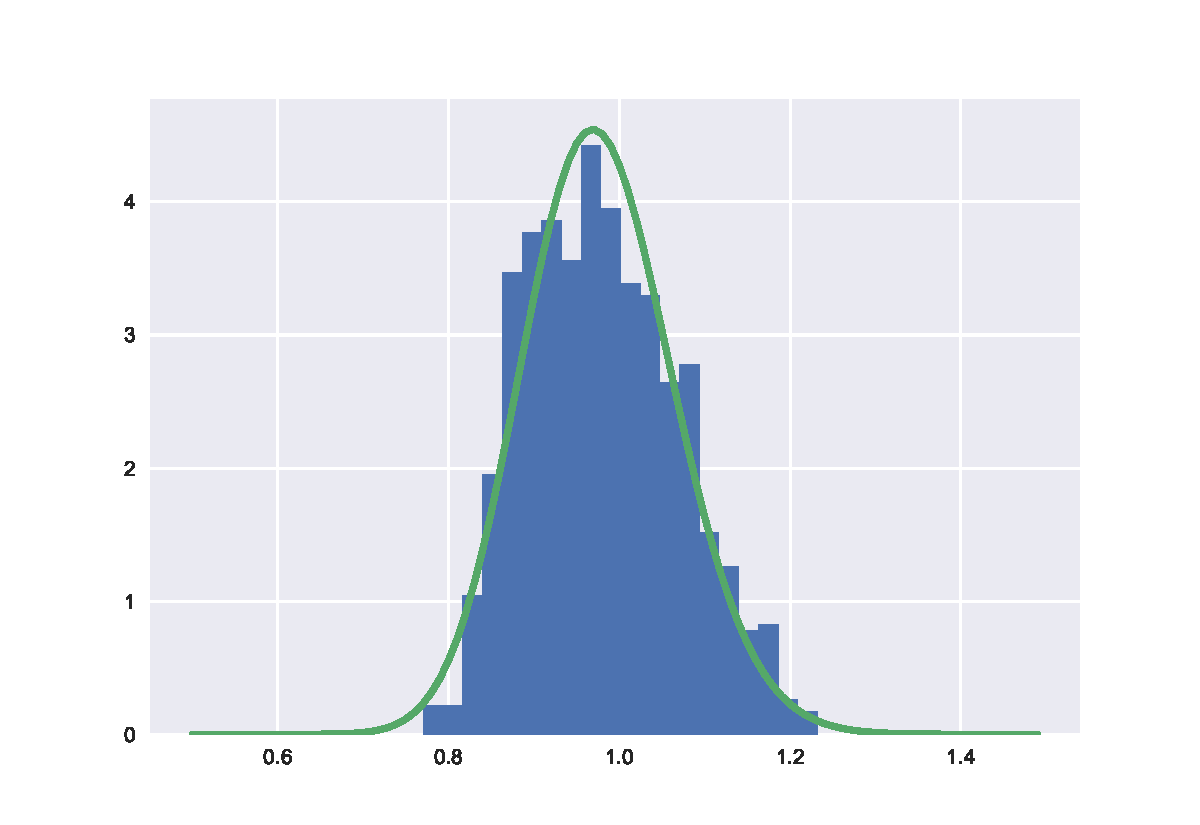
\includegraphics[scale=.4]{mcmc_pic.pdf}
\end{center}
\end{frame}



\begin{frame}%[allowframebreaks]
  \frametitle{References} 
    \bibliographystyle{plainnat}
    \bibliography{finance} %
\end{frame}


\section*{}
\begin{frame}
  \frametitle{$\left.\right.$}
  \begin{center}
    \vspace{1.5cm}
    \large{\bf Thank you!}
    \vspace{2.25cm}
  \end{center}
  \begin{columns}[b]
    \column{.7\linewidth} \scalebox{.75}{ %
      \begin{minipage}{1.2\linewidth}
        {\bf Prof.\ Dr.\ Natalie Packham}\\
        Professor of Mathematics and Statistics\\
        Berlin School of Economics and Law\\
	Badensche Str.\ 52\\
        10825 Berlin
      \end{minipage}
    } %
    \vspace{0pt} \column{.3\linewidth}
    
\includegraphics[width=3cm]{HWR_Logo_RGB.jpg}
    \vspace{0pt}
  \end{columns}
\end{frame}
\end{document}

